\documentclass[dvipsnames]{beamer}
\usetheme{ensam}
\usepackage{pgfplots}
\usepackage{booktabs}
\usepackage{subcaption}
\usepackage{amssymb}
\usepackage{acronym}
\usepackage{mynotations}
\usepackage{tikz}
\usepackage{pgf-pie}
\usetikzlibrary{calc}
\usepackage{amsmath}
\usepackage {algorithmic}
\usepackage{algorithm}
\usepackage{eqparbox}
\usepackage[font=scriptsize]{caption}
\usetikzlibrary{bayesnet,positioning,calc}
\usepgfplotslibrary{groupplots}
\tikzstyle{obs} = [latent,fill=lightBlue]
\tikzstyle{default}=[draw=sexyRed,thick,rounded corners,text width=0.5in,font=\scriptsize,align=center]
\usepgfplotslibrary{colorbrewer}
\definecolor{ForestGreen}{RGB}{34,139,34}
\newcommand{\comment}[1]{\textcolor{ForestGreen}{#1}}
%algorithmic comment
\renewcommand\algorithmiccomment[1]{%
  \hfill\comment{\#\scriptsize\eqparbox{COMMENT}{#1}}%
}
\renewcommand{\algorithmicrequire}{\textbf{Input:}}
\renewcommand{\algorithmicensure}{\textbf{Output:}}
\title{Espaces Vectoriels}
\author{\underline{A.Belcaid}}
\institute{\small Université Euro Méditerranéenne de Fès} 


% Customzation {{{ %
% }}} Customzation %

%tikz bayesian theme
\usetikzlibrary{bayesnet,positioning,calc}
\tikzstyle{obs} = [latent,fill=lightBlue]
\tikzstyle{default}=[draw=sexyRed,thick,rounded corners,text width=0.5in,font=\scriptsize,align=center]
\DeclareMathOperator{\argmin}{argmin}

\pgfplotsset{every tick label/.append style={font=\tiny}}





% add bibliography
\date{\today}

\begin{document}
\maketitle

%{{{ Table de matière
\begin{frame}[t]
  \frametitle{Table de matière}
 \tableofcontents 
\end{frame}
%}}}
% Full document {{{ %
% Introduction Définition {{{ %
\section{Définition}%
\label{sec:définition}
%{{{Importance
\begin{frame}[t]
  \frametitle{Introduction}
  
  \begin{block}{Espace vectoriel}
    \small
    \begin{itemize}
      \item \textbf{\alert{Structure}} commune entre différents objets
        mathématiques\\[10pt]
      \item Obtenir des théorèmes \textbf{généraux}  qui
        s'appliquent non seulement aux \textbf{vecteurs}  mais
        aussi à des fonctions, polynômes ou
        \textbf{matrices}.\\[10pt]
      \item Cette généralité pose une \textbf{difficulté} à
        appréhender ces notions et vous demandera une
        \textbf{\alert{quantité conséquente de travail!}}
    \end{itemize} 
  \end{block}

  \begin{itemize}
    \item Dans le reste de chapitre, $\mathbb{K}$ désigne un corps. Dans la majorité des cas, $$\Kk = \Rr$$ 
  \end{itemize}
\end{frame}
%}}}
% Définition {{{ %
\begin{frame}[<+->]
  \frametitle{Définition}
 
  \begin{block}{Définition}
    \small
    un \alert{$\Kk$-espace vectoriel}  est un ensemble non vide $E$ muni:

    \begin{itemize}
      \scriptsize
      \item Une loi de \textbf{composition interne}, c'est-à-dire
        d'une application de $E \times E$ dans $E$:
        $$
        \begin{array}{lcl}
          E\times E & \rightarrow & E\\
          (A, B)&   \rightarrow & A \alert{\mathbf{+}} B
        \end{array}
        $$
      \item D'une loi \textbf{externe}, c'est-à-dire d'une application
        $\Kk\times E$ dans $E$:

        $$
        \begin{array}{lcl}
          \mathbf{\Kk}\times E & \rightarrow & E\\
          (\lambda, A)&   \rightarrow & \lambda \mathbf{.} 
        \end{array}
$$
    \end{itemize}
  \end{block}
\end{frame}


\begin{frame}[<+->]
  \frametitle{Condition des lois}
  \begin{itemize}
    \small
    \item La loi interne et externe doivent vérifier les conditions
      suivantes:
  \end{itemize} 

  \begin{block}{Condition Loi interne (Groupe)}
 \begin{enumerate}
   \small
 \item  $A + B = B + A\quad\quad \forall A, B \in E$\\[4pt]
 \item $A+(B + C) = (A + B) + C\quad\quad \forall A,B \text{ et  } C\in E$\\[4pt]
 \item il existe un \textbf{\alert{élément neutre}} $0_E$ tel que $ A + 0_E
   = A\quad(\forall A\in E)$
 \item Tout élément  $A\in E$, admet un \textbf{\alert{symétrique}}
   $A^{'}$
   tel que $A + A^{'} = 0_E$
 \end{enumerate} 
\end{block}

\begin{block}{loi Externe}
  \begin{itemize}
    \item $1.A = A\quad (\forall A \in E)$
    \item $\lambda.(\beta.A)  = (\lambda\beta).A\quad(\forall \lambda, \beta
      \in \Kk \text{ et } A \in E)$
    \item $\lambda(A + B) = \lambda.A + \lambda.B\quad (\forall A,B
      \in E \text{ et } \lambda \in \Kk)$
    \item $(\lambda + \beta).A = \lambda.A + \beta.A \quad (\forall
      \lambda, \beta \in \Kk \text{ et } A\in E$.
  \end{itemize} 
\end{block}
\end{frame}
% }}} Définition %
% Examples {{{ %
% The space R2 {{{ %
\begin{frame}[t]
  \frametitle{Exemple (1) $\Rr^{2}$}

\begin{columns}
  \begin{column}{0.4\textwidth}
    
    \begin{center}
    \begin{tikzpicture}[scale=0.35, >=stealth]
    %plans
    \draw[thick, opacity=0.5,->,gray] (-4,0)--(10,0);
    \draw[thick, opacity=0.5,->,gray] (0,-4)--(0,10);
    
    %first drawy
    \draw[sexyRed, thick,->] (0,0)--(4,2)node[pos=0.9, label=below:$A$]{};
    \draw[sexyRed, thick,dotted,->] (0,0)--(8,4)node[pos=0.9, label=below:$2*A$]{};
    \draw[sexyRed, thick,->] (0,0)--(-4,-2)node[pos=0.9, label=below:$-A$]{};
    \draw[lightBlue, thick,->] (0,0)--(2,3)node[pos=0.9, label=left:$B$]{};
    \draw[lightBlue, thick,dotted,->] (0,0)--(4,6)node[pos=0.9, label=left:$2*B$]{};
    \draw[lightBlue, thick,dashed,->] (0,0)--(6,5)node[pos=1, label=right:$A+B$]{};
    \node[circle, fill, minimum width=2pt, inner sep=0pt, label=above left:$0$] at (0,0){};
    \draw[dashed,thick,->](2,3)--(6,5);
    \draw[dashed,thick,->](4,2)--(6,5);
    \end{tikzpicture}
    \end{center}
  \end{column}
  \begin{column}{0.6\textwidth}
    \small
  \begin{itemize}
    \item $E = \left\{ (x, y)\;|\; x\in \Rr\;,\; y \in \Rr\right\}$
      \pause
    \item \textbf{\alert{Loi interne} }
      \begin{equation*}
        \scriptsize
        (x_1, y_1) + (x_2, y_2) = (x_1+ y_1\;, \; x_2 + y_2)
      \end{equation*}
      \pause
    \item \textbf{\alert{Loi externe}} 
      \begin{equation*}
        \lambda \in \Rr, (x,y)\in \Rr^2, \quad \lambda (x,y) = (\lambda x,
        \lambda y)
      \end{equation*}
    \item \textbf{Elément neutre}: $0=(0,0)$ 
  \end{itemize}   
  \end{column}
\end{columns}
\end{frame}
% }}} The space R2 %
% The genreal Space Rn {{{ %
\begin{frame}[<+->]
  \frametitle{Forme générale $\Rr^n$}
  \begin{itemize}
    \small
    \item La généralisation de $\Rr^2$ où chaque élément est un
      \textbf{couple} est \alert{$\Rr^{n}$} où chaque élément un
      \textbf{\alert{n-uplet}} 
      \begin{equation*}
        \Rr^n = \left\{ (x_1,x_2,\ldots, x_n)\;|\; x_i \in \Rr\;\; 1\leq i\leq n \right\}
      \end{equation*}
    \item La loi \textbf{interne} est:

      \begin{equation*}
        (x_1,x_2,\ldots, x_n) + (y_1,y_2,\ldots,y_n) = (x_1 + y_1,
        x_2+y_2,\ldots, x_n+y_n)
      \end{equation*}

    \item \textbf{Loi externe} 
      \begin{equation*}
        \lambda (x_1, x_2,\ldots , x_n)  = (\lambda x_1, \lambda x_2, \ldots,
        \lambda x_n)
      \end{equation*}
  \end{itemize} 
\end{frame}
% }}} The genreal Space Rn %
% Homogenous space {{{ %

\begin{frame}[t]
  \frametitle{Exemple 3: Plan}
 \begin{block}{Plan}
   \small
   Tout \textbf{plan} $\mathcal{P}$ passant par \textbf{\alert{l'origine}} est
   un espace vectoriel (muni des operations habituels de $\Rr^3$.)
 \end{block} 

     \begin{equation*}
       \mathcal{P} = \left\{ (x,y,z) \in \Rr^3\;|\; ax + by +cz=0\right\}
     \end{equation*}

     \begin{itemize}
       \item Vérifier les axioms d'un espace vectoriel.
     \end{itemize}
\end{frame}
% }}} Homogenous space %
% Espace des fonctions {{{ %
\begin{frame}[t]
  \frametitle{Exemple (4): Espace des fonctions}

  \begin{itemize}
    \small
    \item L'ensemble des \textbf{fonctions} de $\Rr$ vers $\Rr$ que nous
      notons $\mathcal{F}(\Rr, \Rr)$.\\[8pt]

    \item \structure{\textbf{Loi interne}}: Pour deux fonctions $f$ et
      $g \in \mathcal{F}(\Rr,\Rr)$.

      \begin{equation*}
        (f+g)(x) = f(x) + g(x)\quad x \in \Rr
      \end{equation*}

    \item \textbf{\structure{Loi externe}}: notée $\times$.

      \begin{equation}
        (\lambda f)(x) = \lambda f(x)
      \end{equation}
    \item \textbf{\structure{Elément neutre}} : 

      \begin{equation*}
        0_{\mathcal{F}}(x) = 0 \quad \forall x\in\Rr
      \end{equation*}

    \item \textbf{\structure{Opposé}} : 

      \begin{equation*}
        (-f)(x) = -f(x) \quad x \in \Rr
      \end{equation*}
  \end{itemize}
\end{frame}
% }}} Espace des fonctions %
% }}} Examples %
% Terminologie {{{ %
\begin{frame}[<+->]
  \frametitle{Terminologie}
  \begin{itemize}
    \item L'espace vectoriel sur $\Kk$ est dit
      \alert{$\Kk$-espace vectoriel}.\\[4pt]
    \item Les éléments de $E$ sont appelés des
      \textbf{\alert{vecteur}}.\\[4pt]

    \item Les éléments de $\Kk$ sont appelés des
      \textbf{\structure{scalaires}}.\\[4pt]
    \item L'élément neutre de la loi interne est $0_E$ est appelé
      \textbf{\alert{vecteur nul}}.\\[4pt]
    \item L'inverse d'un vecteur $A$ dans $E$ est appelé
      \textbf{\alert{opposé}}.\\[4pt]
    \item On se refère à la loi externe par
      \textbf{multiplication}.
  \end{itemize} 
\end{frame}
% }}} Terminologie %
% Règles de calcul {{{ %
\begin{frame}[<+->]
  \frametitle{Règles de calcul}
 Soit $E$ un espace vectoriel sur un corps $\Kk$. Soient $A\in E$ et
 $\lambda\in \Kk$. alors\\[6pt]
  \begin{block}{Proposition}
    \begin{enumerate}
      \small
    \item $0 . A = 0_E$.\\[8pt]

    \item $\lambda.0_E = 0_E$
      (\textbf{\alert{élément absorbant}})\\[8pt]
    \item $(-1).A = -A$ \\[8pt]
    \item $\lambda.A = 0_E \iff \lambda =0 \quad \text{ou}\quad
        A=0_E$
    \end{enumerate}
  \end{block}
  \begin{itemize}
    \item Donner un preuve?
  \end{itemize}
\end{frame}
% }}} Règles de calcul %
% Mini exercice {{{ %
\begin{frame}[t]
  \frametitle{Mini exercice}
  
  \small
  Pour chaque cas, vérifier s'il s'agit d'une \textbf{espace
  vectoriel}?

  \begin{block}{Mini-exercice}
  \begin{enumerate}
    \scriptsize
    \item L'ensemble des fonctions réelles sur $[0,1]$, continues
      positives ou nulles, pour l'\textbf{addition} et le produit par un
      réel.\\[4pt]

    \item L'ensemble des fonctions réelles sur $\Rr$ vérifiant
      $\lim_{x\to \infty} f(x) = 0$ par les mêmes
      opérations.\\[4pt]

    \item L'ensemble $\Rr_{+}^{*}$ pour les opérations 
      \begin{equation*}
        x \oplus y = xy\quad \lambda.x = x^{\lambda}
        (\lambda\in\Rr)
      \end{equation*}
    \item L'ensemble des points $(x,y)$ de $\Rr^{2}$ vérifiant
      \begin{equation*}
        sin(x+y) = 0
      \end{equation*}
    \item L'ensmble des vecteurs $(x,y,z)$ de $\Rr^3$
      \textbf{orthogonaux} au vecteur $(-1,3,-2)$. 
  \end{enumerate}

\end{block}
\end{frame}

% }}} Mini exercice %
% }}} Introduction Définition %
% Sous espace vectoriels {{{ %
\subsection{Sous-espace vectoriel}%
\label{sub:sous_espace_vectoriel}
% Définition {{{ %
\begin{frame}[<+->]
  \frametitle{Sous espace Vectoriel}

  \begin{block}{Définition}
    \small
    Similaire à la notion de groupe. Si on possède un $\Kk$-espace
    vectoriel $E$. Une \textbf{partie}  $F$ de $E$ est appelée un
    \textbf{\alert{sous espace vectoriel}} si:

      \begin{itemize}
        \item $0_E \in F$. (\textbf{élément neutre})\\[10pt]
        \item $A + B \in F\quad \forall A, B \in F$. \structure{Loi
          interne}\\[10pt]

        \item $\lambda.A\in F\quad \forall \lambda\in \Kk \;\text{et}\; A\in F$
          (\textbf{\alert{Loi externe}})
      \end{itemize}
  \end{block}
  
\end{frame}
% }}} Définition %
% Exemples {{{ %
% Droite origine {{{ %
\begin{frame}[t]
  \frametitle{Exemple (1)}

  \begin{block}{Droite passant par l'origine}
    \small
   \begin{equation*}
     \small
     \mathcal{D} = \left\{(x,y)\;|\; 3x - 2y = 0\right\}
   \end{equation*} 
  \end{block}
  \begin{figure}[htpb]
  \begin{center}
  \begin{tikzpicture}[scale=1, transform shape]
    \begin{axis}[width=10cm, height=6cm, axis lines=center]
      \addplot[sexyRed,thick]{-1.5*x}; 
      \addlegendentry{$\mathcal{D}$}
   \end{axis} 
  \end{tikzpicture}
  \end{center}
  \caption{Droite passant par l'origine}%
  \label{fig:}
  \end{figure}
  
  
\end{frame}
% }}} Droite origine %
% D'autre exemples {{{ %
\begin{frame}[t]
  \frametitle{Exemple (2)}
  
  \begin{block}{Sous groupes ?}
    \begin{itemize}
      \small
      \item $$F_1 =\left\{(x,y)\in \Rr^2\;|\; x + y= 2\right\}$$

      \item $$F_2 = \left\{(x,y)\in \Rr^2\;|\; x=0\;\text{ou } y=
        0\right\}$$
    \item $$F_3 = \left\{(x,y)\in \Rr^2\;|\; x\geq0\;\text{et } y\geq
        0\right\}$$
    \end{itemize} 
  \end{block}

  \begin{figure}[htpb]
  \begin{center}
  \begin{tikzpicture}[scale=0.7, >=latex]
    \begin{groupplot}[group style={group size= 3 by 1},height=5cm,width=5cm]
      \nextgroupplot[title=$F_1$,axis lines=center]
      \plot[thick, sexyRed]{2-x};
      \nextgroupplot[title=$F_2$,axis
      lines=center,ymin=-1,ymax=4,xmin=-1,xmax=4]
      \path[very thick, sexyRed,draw](axis cs:-2,0)--(axis cs:4,0);

      \path[very thick, sexyRed,draw](axis cs:0,-1)--(axis cs:0,4);
      \node (F) at (axis cs:1,1){$F_2$};
      \path[draw, ->] (F)--(axis cs:1,0);
      \path[draw, ->] (F)--(axis cs:0,1);
      \nextgroupplot[title=$F_3$,xmin=-2,ymin=-2,ymax=5,xmax=5,axis lines=center]

      \fill[sexyRed, draw,opacity=0.5] (axis cs:0,0) rectangle (axis cs: 5,5);
      \node at (axis cs:2,2) {$F_3$};
    \end{groupplot}
  \end{tikzpicture}
  \end{center}
  \caption{}%
  \label{fig:}
  \end{figure}
\end{frame}
% }}} D'autre exemples %
% Vérification simple {{{ %
\begin{frame}[t]
  \frametitle{Exemples (2) Vérification}
  Pour chaque cas, vérifier s'il s'agit d'un espace vectoriel


  \begin{block}{Mini Exercice}
    \begin{enumerate}
      \small
      \item L'ensemble des fonction \textbf{paires}.\\[6pt]

      \item L'ensemble des fonctions \textbf{impaires}.\\[6pt]

      \item
        \begin{equation*}
          E=\left\{(x,y,z,t)\in\Rr^4\;|\; x=t\;\text{et}\; y=z\right\}
        \end{equation*}
      \item 
        \begin{equation*}
          E=\{(x,y)\in \Rr^2\;|\; x^2 + xy\geq 0\}
        \end{equation*}
      \item 
        \begin{equation*}
          E = \{f\in \mathcal{F}(\Rr,\Rr)\;|\; f \text{ est
          croissante}\}
        \end{equation*}
      \item 
\begin{equation*}
  \left\{(u_n)_{n\in\Nn}\;|\; (u_n)\to 0\right\}
\end{equation*}
    \end{enumerate}
  \end{block}
  
\end{frame}
% }}} Vérification simple %
% }}} Exemples %
% Span {{{ %
\begin{frame}[t]
  \frametitle{Combinaison Linéaire}
     \small
    \begin{block}{Définition}
      Soient $B_1, B_2,\ldots, B_n$ des vecteurs d'un espace vectoriel
      $E$. On appelle une \textbf{\alert{combinaison linéaire}} des
      $(B_i)_{1,n}$ est un \textbf{vecteur}:
      \begin{equation}
        V = \lambda_1 B_1 + \lambda_2B_2\ldots + \lambda_n B_n
      \end{equation}
    \end{block} 

    \begin{itemize}
      \small
      \item Si $n=1$, alors $V=\lambda B$. on dit alors que $V$ et $ B$
        sont \textbf{\alert{colinéaire}}. 
    \end{itemize}
    \begin{center}
    \begin{tikzpicture}[scale=0.5, >=latex]
      \draw[gray,very thick,->] (-2,0)--(6,0);
      \draw[gray,very thick,->] (0,-2)--(0,6);
      \node (A) at (4,1) {$A$};
      \node (B) at (1,2) {$B$};
      \node (C) at (2,4) {$2B$};
      \node (D) at (6,5) {$A+2B$};
      \draw[thick, sexyRed,->, draw] (0,0)--(B);
      \draw[thick, sexyRed,->, draw] (0,0)--(A);
      \draw[thick,->, draw] (0,0)--(D);
      \draw[thick, lightBlue,->, draw,opacity=0.5] (0,0)--(C);
      
    \end{tikzpicture}
    \end{center}
    
\end{frame}

% }}} Span %
% Exemples {{{ %
\begin{frame}[t]
  \frametitle{Exemples}
 \begin{block}{Exemples}

   \begin{enumerate}
     \small
   \item Dans $\Rr^3$, $(4,1,3)$ est une combinaison linéaire de
     $(1,0,1)$ et $(0,1,0)$ car:
     $$
     (4,1,4) = 4(1,0,1) + 1(0,1,0)
     $$

   \item Est ce que le vecteur $(2,1)$ est \textbf{collinéaire}
     avec $(1,0)$?

   \item On considère l'espace $E=\mathcal{F}(\Rr,\Rr)$, on considère les
     monômes 
     \begin{equation*}
       \forall x\in \Rr,\quad f_0(x)=1,\;f_1(x)=x,\; f_2(x)=x^2,\;
       f_3(x)=x^3
     \end{equation*}
     alors la fonction $f(x) = x^3 -2x^2 -7x -4$ peut s'écrire comme
     une combinaison linéaire des $(f_i)$ 
     \begin{equation*}
       f(x) = f_3 -2f_2 - 7f_1 -4f_0
     \end{equation*}
   \end{enumerate}
 \end{block} 
\end{frame}
% }}} Exemples %
% Recherche Coefficients {{{ %
\begin{frame}[t]
  \frametitle{Recherche Coefficients}
  \begin{block}{Exemple (1)}
    \small
    Soit $u=(1, 2, -1)$ et $v= (6,4,2)$ deux vecteurs de $\Rr^3$. Montrons
    que $w=(9,2,7)$ est une combinaison linéaire de $u$ et $v$.
    % \pause

    \begin{equation*}
      \small
      \begin{pmatrix}
        9\\2\\7
        \end{pmatrix} = \lambda \begin{pmatrix}1\\2\\-1\end{pmatrix}
        + \beta \begin{pmatrix}6\\4\\2\end{pmatrix}=
        \begin{pmatrix}\lambda + 6\beta\\ 2\lambda + 4\beta \\
        -\lambda + 2\beta\end{pmatrix}
    \end{equation*}
    Ainsi on trouve:

    \begin{equation*}
      \left\{ \begin{array}{lll} 9 &=& \lambda + 6\beta\\ 2&=& 2\lambda +
      4\beta\\7&=&-\lambda + 2\beta\end{array}\right.
    \end{equation*}
    On retrouve que \alert{$\lambda=-3,\; \beta=2$}
\pause

\begin{block}{Exemple (2)}
  Reprenez la même procédure pour $u=(1,2,-1)$, $v=(6,4,2)$ et $w=(4,-1,8)$.
  
\end{block}
  \end{block}

\end{frame}
% }}} Recherche Coefficients %
% Caractérisation {{{ %
\begin{frame}[t]
  \frametitle{Caractérisation d'un sous espace}
 \begin{block}{Caractérisation Sous espace vectoriel}
   \small
   Soient $E$ un $\Kk$-espace vectoriel et $F$ une \textbf{partie} non
   vide de $E$. $F$ est un sous espace vectoriel \textbf{si et
   seulement si}:

   \begin{equation}
     \underComment{\lambda U + \mu V}{\scriptsize combinaison
     linéaire} \in F \quad \forall U,V\in F \quad \forall
     \lambda,\mu \in \Kk
   \end{equation}
 \end{block} 
 \begin{itemize}
   \item Donner une preuve
 \end{itemize}
\end{frame}
% }}} Caractérisation %
% Intersection {{{ %
\begin{frame}[t]
  \frametitle{Intersection}
  \begin{block}{Proposition}
    \small
    Soient $F$ et $G$ deux sous-espace vectoriel d'un $\Kk$-espace
    vectoriel. L' \textbf{intersection} \alert{$F\cap G$} est aussi un espace
    vectoriel.
  \end{block}

  \begin{itemize}
    \item Donner une preuve?
  \end{itemize}

      \begin{block}{Exemple}
      \scriptsize
      $$
        \mathcal{D}=\left\{(x,y,z)\in\Rr^3\;\; x+3y+z=0\;\text{et}\;
        x-y+2z=0\right\}$$ 
      \end{block}
\scriptsize
      On peut considérer 
$$
\left\{
\begin{array}{lll}
  F&=&\{(x,y,z)\in\Rr^3\;|\; x+3y+z=0\}\\
  G&=&\{(x,y,z)\in\Rr^3\;|\; x-y+2z=0\}
\end{array}
\right.
$$
\end{frame}
% }}} Intersection 
% Union {{{ %
\begin{frame}[t]
  \frametitle{Union}
  
  \begin{block}{Remarque}
    \small
    Malheureusement, \textbf{L'union}  de deux sous espaces vectoriels
    \textbf{\alert{n'est}} pas un sous espace vectoriel. 
  \end{block}

  \begin{block}{Contre exemple}
    \small
    \begin{equation*}
      \left\{\begin{array}{l}
          F = \{(x,y)\;|\; x=0\}\\[6pt]
          G = \{(x,y)\;|\; y=0\}\\[6pt]
          (0,1)\in F\cup G\text{ et  } (1,0)\in F\cup G \;\text{mais } (1,1) \notin
          F\cap G
      \end{array}\right.
    \end{equation*}
  \end{block}

  \begin{center}
    \begin{tikzpicture}[scale=0.4,>=stealth]
      \path[gray,draw, very thick, ->,opacity=0.5](-2,0)--(6,0);
      \path[gray,draw, very thick, ->,opacity=0.5](0,-2)--(0,6);
      \node[sexyRed,label=right:$F$] (F) at (3,0){};
      \node[sexyRed,label=right:{$(1,1)$}] (S) at (2,2){};
      \node[sexyRed,label=above:$G$] (G) at (0,3){};
      \draw[sexyRed,thick] (0,0)--(F);
      \draw[sexyRed,thick] (0,0)--(G);
      \draw[->,thick](0,0)--(S);
    \end{tikzpicture}
\end{center} 
  % \end{block}
\end{frame}
% }}} Union %
% Somme directe {{{ %
\begin{frame}[t]
  \frametitle{Somme directe}

  \begin{block}{Somme directe}
    \small
    Si on cherche un espace vectortiel qui contient $F$ et $F$. On définit
    la \textbf{\alert{somme directe}} de $F$ et $G$

    \begin{equation}
      F+G = \left\{u+v\;|\; u\in F,\; v\in G\right\}
    \end{equation}
  \end{block}
  \begin{figure}[htpb]
  \begin{center}
  \begin{tikzpicture}[scale=0.6, transform shape]
    \path[thick, lightBlue,draw](-2,0)--(4,0);    
    \node at (4.2,0) {F};
    \path[thick, lightBlue,draw](-2,-2)--(1,4);    
    \node at (1,4.3) {G};
    \node at (2,2) {F+G};
    \path[fill,sexyRed, opacity=0.5](-3,-2)--(3,-2)--(6,4)--(-0,4)--cycle;
  \end{tikzpicture}
  \end{center}
  \caption{Somme directe }%
  \label{fig:}
  \end{figure}
\end{frame}


% Minimal space {{{ %
\begin{frame}[<+->]
  \frametitle{Propriété Somme directe}
 \begin{block}{Proposition}
   Soient $E$ e $F$ deux \textbf{sous-espaces} vectoriels  d'un $\Kk$-espace
   vectoriel.\\[8pt]

   \begin{enumerate}
     \small
     \item  $F + G$ est \textbf{\alert{sous espace}} vectoriel.\\[6pt] 
     \item  $F + G$ est \textbf{\alert{ le plus petit}} sous espace vectoriel
       contenant à l fois $F$ et $G$. 
   \end{enumerate}
 \end{block} 

 \begin{block}{Exemple}
   \small

   \begin{equation*}
     \left\{\begin{array}{lll}
         F &=& \left\{(x,y,z)\in\Rr^3 \;|\; x=0\right\}\\[6pt]
         G &=& \left\{(x,y,z)\in\Rr^3 \;|\; y=0\right\}
     \end{array}\right.
   \end{equation*}

   Déterminer l'espace vectoriel $$F+ G$$.
 \end{block}
\end{frame}
% }}} Minimal space %
% Somme supplémentaire {{{ %
\begin{frame}[t]
  \frametitle{Somme supplémentaire}
 \begin{block}{Somme directe}
   \small
  Soient $F$ et $G$ deux sous espaces vectoriels de $E$. $F$ et $G$ sont en
  \textbf{\alert{somme directe}} si:

  \begin{enumerate}
    \item $F\cap G = \left\{0_E\right\}$\\[4pt]
    \item $F + G = E$.
  \end{enumerate}
  Dans ce cas on dit que $F$ et $G$ sont \textbf{\alert{supplémentaires}} et on
  écrit:

\begin{equation}
  E = F \oplus G
\end{equation}
 \end{block} 

 \begin{block}{Proposition}
   \small
  $F$ et $G$ sont supplémentaires dans $E$ si tout élément de $E$ s'écrit
  d'une manière \textbf{\alert{unique}} comme la somme d'un élément de $F$
  et d'un élément de $G$.

 \end{block}
\end{frame}
% }}} Somme supplémentaire %
% Exemple Supplémentaires {{{ %
\begin{frame}[<+->]
  \frametitle{Exemple Espaces supplémentaires}

  \begin{block}{Exemple 1}
    \small
   \begin{equation*}
     \left\{\begin{array}{lll}
         F & = & \left\{(x,y) \in \Rr^2\;|\; x=0\right\}\\[6pt]
         G & = & \left\{(x,y) \in \Rr^2\;|\; y=0\right\}
     \end{array}\right.
   \end{equation*} 
   prouver que $$ \Rr^2 = F \oplus G$$
  \end{block}
 
\begin{block}{Exemple 2}
  \small
  Même question dans $\Rr^3$ pour 

   \begin{equation*}
     \left\{\begin{array}{lll}
         F & = & \left\{(x,y,z) \in \Rr^3\;|\; x-y-z=0\right\}\\[6pt]
         G & = & \left\{(x,y,z) \in \Rr^3\;|\; y=z=0\right\}
     \end{array}\right.
   \end{equation*} 
\end{block}
\end{frame}
% }}} Exemple Supplémentaires %
% }}} Somme directe %
% Span of vecttors {{{ %
\begin{frame}[<+->]
  \frametitle{Sous espace engendré}
 \begin{block}{Théorème}
   \small
   Soient $\left\{v_1,v_2,\ldots,v_n\right\}$ un ensemble fini de vecteurs dans
   un $\Kk$-espace vectoriel $E$ alors:

   \begin{itemize}
     \item L'ensemble des \textbf{\alert{combination linéaires}} de
       $\{v_1,\ldots,v_n\}$ est un \textbf{sous espace vectoriel} de $E$.\\[4pt]
     \item C'est \alert{le plus petit} sous espace vectoriel contenant les vecteurs
       $v_1,v_2,\ldots, v_n$.
   \end{itemize}
 \end{block} 

 Cet espace est appelé espace \textbf{engendré}  par $v_1,\ldots,v_n$:
 \begin{equation}
   \text{Vect}(v_1,\ldots,v_n) = \big\{ \sum_{i=0}^n \lambda_i v_i\;|\; \lambda_i \in
   \Kk\big\}
 \end{equation}
\end{frame}
% }}} Span of vecttors %
% Examples Spans {{{ %
\begin{frame}[<+->]
  \frametitle{Exemples Espace Engedré}
 \begin{columns}
   \begin{column}{0.5\textwidth}
     \begin{itemize}
       \scriptsize
       \item Si $u$ est un vecteur d'un espace vectoriel $E$, 
         \begin{equation*}
           \text{Vect}(u)  = \left\{\lambda u\;|\; \lambda \in \Kk \right\}=\Kk
           u
         \end{equation*}
         \begin{figure}[htpb]
         \begin{center}
         \begin{tikzpicture}[scale=0.7, transform shape]
           \path[draw, thick, sexyRed] (-3,-3)--(3,3); 
           \path[draw, thick,thick,->,>=latex, lightBlue]
             (0,-0.2)--(1,0.8)node[label=below:$u$]{}; 
           \node[minimum width=5pt,fill,circle, inner sep=0pt,label=left:$0_E$] (O) at (0,0) {};
         \end{tikzpicture}
         \end{center}
         \caption{Droite vectotielle}%
         \label{fig:}
         \end{figure}
         
     \end{itemize} 
   \end{column}
   \pause
   \begin{column}{0.5\textwidth}
     
     \scriptsize 
     Si $u$ et $v$ sont deux vecteurs de $E$, on définit un \textbf{\alert{plan
     vectoriel}}  par:

     \begin{equation*}
       \text{Vect}(u,v)  = \left\{ \lambda u + \mu v \;|\; \lambda, \mu \in \Kk
       \right\}
     \end{equation*}


     \begin{figure}[htpb]
     \begin{center}
     \begin{tikzpicture}[scale=0.6, transform shape]
       \path[fill, sexyRed, opacity=0.8] (0,0)--(3,3)--(0,6)--(-3,3)--cycle; 
        \node[minimum width=5pt,fill,circle, inner sep=0pt,label=left:$0_E$] (O) at (0,0) {};

           \path[draw, thick,thick,->,>=latex]
             (0,3)--(1,4)node[label=below:$u$]{}; 

           \path[draw, thick,thick,->,>=latex ]
             (0,3)--(1,2)node[label=below:$v$]{}; 
     \end{tikzpicture}
     \end{center}
     \caption{Plan vectoriel}%
     \label{fig:}
     \end{figure}
     
   \end{column}
 \end{columns} 
\end{frame}
% }}} Examples Spans %
% Exemple Span 2 {{{ %
\begin{frame}[<+->]
  \frametitle{Exemple 2}
  \begin{block}{Exemple Polynomes}
    \small
  L'ensemble 
  \begin{eqnarray*}
    \mathcal{P}_2 &=& \left\{ P \in \Rr[X]\;|\; \text{deg}(P) = \mathbf{2}
    \right\}\\[4pt]
    \mathcal{P}_2 &=& \left\{P \in \Rr[X]\;|\; P= aX^2 + bX + c\right\}\\
    \mathcal{P}_2 &=& \text{Vect}(X^2, X, 1)
\end{eqnarray*}
 \end{block} 
 \begin{block}{Exemple 3}
   \small
  \begin{eqnarray*}
    F &=& \left\{ (x,y,z) \in \Rr^3\;|\; x - y -z = 0 \right\}\\[4pt]\pause
    F &=& \left\{ (x,y,z) \in \Rr^3\;|\; (y+z, y, z) \right\}\\[4pt]\pause
    F &=& y(1,1,0) + z(1,0,1)\\[4pt]\pause
    F &=& \text{Vect}\left(\left(1,1,0\right), \left(1,0,1\right)\right)
  \end{eqnarray*} 
 \end{block}
\end{frame}
% }}} Exemple Span 2 %  
% }}} Sous espace vectoriels %
% Applications linéaires {{{ %
\subsection{Applications Linéaires}%
\label{sub:applications_linéaires}

% Applications linéaires {{{1 %
% Définition {{{ %
\begin{frame}[<+->]
  \frametitle{Définition}
 \begin{block}{Définition}
   \small
   Soient $E$ et $F$ deux espace vectoriels. Une application $f: E\rightarrow F$
   est une \textbf{\alert{application linéaire}} si elle satisfait les deux
   conditions suivantes:

   \begin{enumerate}
     \item $\forall u, v \in E\quad f(u + v) = f(u) + f(v)$\\[6pt]
     \item $\forall u\in E, \lambda\in \Kk\quad f(\lambda u) = \lambda f(u)$
   \end{enumerate}
 \end{block} 

 \begin{itemize}
   \small
 \item  Une application linéaire doit \textbf{\alert{respecter}}  les deux lois
   d'un espace vectotiel.\\[4pt]
 \item L'ensemble des applications linéaires de $E$ vers $F$ est noté
   \alert{$\mathcal{L}(E,F)$}\\[4pt]
 \item $f$ est aussi appelé un \textbf{\alert{morphisme}} d'espace
   vectoriel.\\[4pt]
 \item Une application $f$ de $E$ vers $\mathbf{E}$ est appelé un
   \textbf{\alert{endomorphisme}} de $E$.
 \end{itemize}
\end{frame}
% }}} Définition %
% Exemples Applicaiton linéaire {{{ %
\begin{frame}[<+->]
  \frametitle{Exemples}
 \begin{block}{Exemple}
   \small
   Soit l'application $f$ définie par

   \begin{equation*}
     \begin{array}{llcl}
       f & \Rr^3 & \rightarrow & \Rr^2\\
         & (x,y,z)& \rightarrow & (-2x, y+ 3z)
    \end{array}
   \end{equation*}
   Vérifier que $f \in \mathcal{L}(\Rr^3, \Rr^2)$.
 \end{block} 
 \begin{block}{Exemple 2}
  L'application 
   \begin{equation*}
     \begin{array}{llcl}
       g & \Rr & \rightarrow & \Rr\\
         & x& \rightarrow & x^2 
    \end{array}
   \end{equation*}
   est-elle linéaire?
 \end{block}
\end{frame}
% }}} Exemples Applicaiton linéaire %
% Propriétés {{{ %
\begin{frame}[<+->]
  \frametitle{Propriétés d'une applicaiton linéaire}
 \begin{block}{Proposition}
   \small
   Soit $f \in \mathcal{L}(E, F)$  alore on as:

   \begin{itemize}
     \item $f(0_E) = 0_F$\\[4pt]
     \item $f(-u)  = -f(u)\quad \forall u\in E$
   \end{itemize}
 \end{block} 

 \begin{block}{Caractérisation d'une application linéaire}
   \small
   Une méthode plus \textbf{concentrée}   pour vérifier que $f\in
   \mathcal{L}(E,F)$ est de prouver que 
   \begin{equation}
     f(\lambda u + \mu v) = \lambda f(u) + \mu f(v) 
   \end{equation}
 \end{block}
 \pause
 \begin{block}{Préservation combinaison linéaire}
   \small
   \begin{equation}
     f\big(\sum_{i=0}^n \lambda_i v_i\big) = \sum_{i=0}^n \lambda_i f(v_i) 
 \end{equation}
 \end{block}
\end{frame}
% }}} Propriétés %
% Mini Exercice {{{ %
\begin{frame}[t]
  \frametitle{Mini Exercice}
 \begin{block}{Mini exercice}
   Pour chaque cas, vérifier si $f_i$ est une applicaiton linéaire
   \begin{enumerate}
     \item $$f_1(x,y) = (-x, -y)$$
     \item $$f_2(x,y) = (3x, 3y)$$
     \item $$f_3(x,y) = (x, y)$$
     \item $$f_4(x,y) = \big(\frac{\sqrt{3}}{2}x -
       \frac{1}{2}y\;\;,\;\; \frac{1}{2}x + \frac{\sqrt{3}}{2}y\big)$$


   \end{enumerate}
 \end{block} 
\end{frame}
% }}} Mini Exercice %
% Exemples Géométriques {{{ %
\begin{frame}[<+->]
  \frametitle{Transformation géométrique}
  \begin{block}{Symétrie centrale}
    \small
    La \textbf{\alert{symétrie centrale}} par rapport à $0_E$  dans un espace vectoriel $E$ est
    définit comme suit:

    \begin{equation}
      \label{eq:central_symmetry}
      \begin{array}{llll}
        f: & E &\longrightarrow & E\\
           & u &\longrightarrow & \alert{-u}
      \end{array}
    \end{equation}
  \end{block}
  \pause
  \begin{figure}[htpb]
  \begin{center}
  \begin{tikzpicture}[scale=0.6,>=latex]
    \path[draw, ->, very thick, gray, opacity=0.8] (-4,0)--(4,0);  
    \path[draw, ->, very thick, gray, opacity=0.8] (0,-4)--(0,4);  
    \path[draw, sexyRed, opacity=0.8,->,thick] (0,0)--(1,2)node[label=above:$u$]{};
    \path[draw, Peach, opacity=0.8,->,very thick](0,0)--(-1,-2)node[label=below:$-u$]{};
  \end{tikzpicture}
  \end{center}
  \caption{Symétrie par rapport au centre}%
  \label{fig:}
  \end{figure}
\end{frame}
\begin{frame}{Homotétie}
  \begin{block}{Homotétie}
    \small
    L'\textbf{\alert{homotétie}} de rapport $\lambda$ d'un espace vectoriel est
    définit comme suit:
    \begin{equation}
      \label{eq:central_symmetry}
      \begin{array}{llll}
        f: & E &\longrightarrow & E\\
           & u &\longrightarrow & \alert{\lambda}.u
      \end{array}
    \end{equation}
    \pause
    \begin{figure}[htpb]
    \begin{center}
    \begin{tikzpicture}[scale=0.7, >=latex]
    \path[draw, ->, very thick, gray, opacity=0.8] (-1,0)--(4,0);  
    \path[draw, ->, very thick, gray, opacity=0.8] (0,-1)--(0,4);  
    \path[draw, sexyRed, opacity=0.8,->,thick] (0,0)--(1,2)node[label=above:$u$]{};
    \path[draw, Peach, opacity=0.8,->,very thick, opacity=0.8](0,0)--(2,4)node[label=below:$2u$]{};
    \path[draw, Peach, opacity=0.8,->,very
      thick, opacity=0.8](0,0)--(0.5,1)node[label=below:$\frac{1}{2}u$]{};
    \end{tikzpicture}
    \end{center}
    \caption{Représentation Homotétie}%
    \label{fig:}
    \end{figure}
    
  \end{block}
\end{frame}


\begin{frame}{Homotétie}
  \begin{block}{Homotétie}
    \small
    L'\textbf{\alert{homotétie}} de rapport $\lambda$ d'un espace vectoriel est
    définit comme suit:
    \begin{equation}
      \label{eq:central_symmetry}
      \begin{array}{llll}
        f: & E &\longrightarrow & E\\
           & u &\longrightarrow & \alert{\lambda}.u
      \end{array}
    \end{equation}
    \pause
    \begin{figure}[htpb]
    \begin{center}
    \begin{tikzpicture}[scale=0.7, >=latex]
    \path[draw, ->, very thick, gray, opacity=0.8] (-1,0)--(4,0);  
    \path[draw, ->, very thick, gray, opacity=0.8] (0,-1)--(0,4);  
    \path[draw, sexyRed, opacity=0.8,->,thick] (0,0)--(1,2)node[label=above:$u$]{};
    \path[draw, Peach, opacity=0.8,->,very thick, opacity=0.8](0,0)--(2,4)node[label=below:$2u$]{};
    \path[draw, Peach, opacity=0.8,->,very
      thick, opacity=0.8](0,0)--(0.5,1)node[label=below:$\frac{1}{2}u$]{};
    \end{tikzpicture}
    \end{center}
    \caption{Représentation Homotétie}%
    \label{fig:}
    \end{figure}
    
    
  \end{block}
\end{frame}

\begin{frame}{Projection}
  \begin{block}{Projection}
    \small
    Si  $F$ et $G$ sont deux sous espace vectoriels \textbf{complémentaires}
    dans $E$. Alors on peut définir deux \textbf{\alert{projections}} $P_F$ et
    $P_G$ donnés comme: Pour chaque $u\in E$ on as $u=v + w$.\\
    \begin{equation}
      \label{eq:central_symmetry}
      \begin{array}{ccc}
        P_F:E \longrightarrow  \mathbf{F} &\quad & P_G : E \longrightarrow
        \mathbf{G} \\
        u   \longrightarrow  \alert{v}  & \quad & u \longrightarrow
        \alert{w}
      \end{array}
    \end{equation}
    \pause
    
  \end{block}

    \begin{figure}[htpb]
    \begin{center}
    \begin{tikzpicture}[scale=0.6, >=latex]
      \draw[very thick, sexyRed, ->] (-2,0) -- (8,0)node[label=right:$F$]{};
      \draw[very thick, sexyRed, ->] (-2,-2) -- (4,4)node[label=left:$G$]{};
      \draw[thick, ->] (0,0) -- (5,2)node[label=above:{$u$}]{};
      \draw[thick, dashed, lightBlue] (5,2)--(2,2);
      \draw[thick, dashed, lightBlue] (5,2)--(3,0);
      \node at (1.2,2) {\small$P_G(u)$};
      \node at (3,-0.9) {\small$P_F(u)$};
    \end{tikzpicture}
    \end{center}
    \caption{Projection Espace Supplémentaires}%
    \label{fig:}
    \end{figure}
\end{frame}
% }}} Exemples Géométriques %
% Mini Exercice {{{ %
\begin{frame}[t]
  \frametitle{Mini Exercice}
  \begin{block}{Mini Exercice}
    \small
    Pour chaque exemple, vérifier si l'application est
    \textbf{linéaire} 

    \begin{enumerate}
      \item
      \begin{equation}
        \begin{array}{lll}
          \Rr & \longrightarrow & \Rr\\
          x   & \longrightarrow & 3x - 2
        \end{array}
      \end{equation}

      \item
      \begin{equation}
        \begin{array}{lll}
          \Rr^4 & \longrightarrow & \Rr\\
          (x_1,x_2,x_3,x_4)   & \longrightarrow & x_1x_3 + x_2x_4
        \end{array}
      \end{equation}

      \item
      \begin{equation}
        \begin{array}{lll}
          \mathcal{C}^1(\Rr,\Rr) & \longrightarrow &
          \mathcal{C}^0(\Rr,\Rr)\\
          f   & \longrightarrow & f + f^{`}
        \end{array}
      \end{equation}

      \item
      \begin{equation}
        \begin{array}{lll}
          \mathcal{C}^0(\Rr,\Rr) & \longrightarrow &
          \mathcal{C}^0(\Rr,\Rr)\\
          f   & \longrightarrow & \max\big(f(x)\big)
        \end{array}
      \end{equation}
    \end{enumerate}

  \end{block}
  
\end{frame}
% }}} Mini Exercice %
% Image d'une application linéaire {{{ %
\begin{frame}[t]
  \frametitle{Image d'une application linéaire}
 \begin{block}{Image d'une application linéaire}
   \small
   Soientt $E$ et $F$ deux espaces vectoriels et $f: E\longrightarrow F$ une
   application linéaire, alors on définit \textbf{\alert{l'image directe}} de
   $E$ par:
   \begin{equation*}
     \text{Im}f = \left\{ f(x) \in F\;|\; x \in E\right\}
   \end{equation*}

   alors on a $\text{Im}f$ est un \textbf{sous espace vectoriel}  de $F$.
 \end{block} 


 \begin{block}{Résultats}
   \small
   \begin{itemize}
     \item Si $E^{'}$ est un sous espace vectoriel de $E$ alors, $\text{Im}E^{'}$
       est aussi un \textbf{\alert{sous espace}} vectoriel de $F$. \\[8pt]

      \item 
        \begin{equation*}
          f  \text{ est surjective} \iff \text{Im}f = F
        \end{equation*}
   \end{itemize}
 \end{block}
\end{frame}
% }}} Image d'une application linéaire %
% Noyau d'une applicaiton linéaire {{{ %
\begin{frame}[t]
  \frametitle{Noyau d'une application linéaire}
  
  \begin{block}{Noyau}
    \small
    Soit $E$ et $F$ deux espaces vectoriels et soit $f:E\longrightarrow F$ une
    application linéaire. On appelle \textbf{\alert{noyau}}  de $f$ noté
    $\text{Ker}(f)$ 

\begin{equation}
  \text{Ker}(f) =\left\{ u \in E\;|\; f(u) = 0_F \right\} 
\end{equation}

  \end{block}
\pause
  \begin{block}{Proposition}
    \small
    Si $E$ et $F$ deux espaces vectoriels et $f: E\longrightarrow F$ une
    application linéaire. Alors $\text{Ker}(f)$ est un \textbf{\alert{sous
    espace vectoriel}}  de $E$.
  \end{block}
  \pause
  \begin{block}{Exemple}
    \small
    Calculer le noyau de 
    \begin{equation*}
      \begin{array}{llll}
        f: &\Rr^3 &\longrightarrow & \Rr^2\\[4pt]
        &   (x,y,z)&\longrightarrow & (-2x,y + 3z)
      \end{array}
    \end{equation*}
  \end{block}
\end{frame}
% }}} Noyau d'une applicaiton linéaire %
% }}} Applications linéaires %
%{{{ Dimension finie
\section{Dimension finie}%
\label{sec:dimension_finie}
% Famille libre {{{ %
\subsection{Famille libre}
\begin{frame}[t]
  \frametitle{Famille libre}
  \begin{block}{Introduction}
    \small
    \begin{itemize}
      \item Les espaces vectoriels qui sont engendrés par un nombre \textbf{fini} de
    vecteurs sont appelés des espaces vectoriels de dimension finie.
  \item Le but de cette section est de savoir comment calculer une
    \textbf{\alert{base}}  pour cet espace.
    \end{itemize}
  \end{block}
  
  \begin{block}{Famille libre}
    \small
    Une famille $\left\{v_1,v_2,\ldots, v_p\right\}$ où $p\geq1$ est dite
    \textbf{\alert{famille libre}}   si toute combinaison linéaire
    \textbf{nulle} :
    \begin{equation*}
     \lambda_1 v_1 + \lambda_2 v_2 + \ldots \lambda_p v_p = 0 
    \end{equation*}
    n'admet qu'une seule solution

    \begin{equation*}
      \lambda_1= 0 \;\; \lambda_2 = 0 \;\; \ldots \lambda_p = 0
    \end{equation*}
  \end{block}
  \begin{itemize}
    \item Dans le cas contraire, on dit que la famille est \textbf{\alert{liée}} 
  \end{itemize}
\end{frame}


\begin{frame}[t]
  \frametitle{Exemple}
 \begin{block}{Exemple }
  On considère dans $\Rr^3$ la famille:
  \begin{equation*}
    \Big\{ 
      \begin{pmatrix}
       1\\2\\3 
      \end{pmatrix}
      ,
      \begin{pmatrix}
       4\\5\\6 
      \end{pmatrix}
      ,
      \begin{pmatrix}
       2\\1\\0 
      \end{pmatrix}
    \Big\}
  \end{equation*}
 \end{block} 

 \small
 On veut vérifier si cette famille est \textbf{libre} ou non?
 \begin{equation*}
   \lambda_1 (1,2,3) + \lambda_2(4,5,6) + \lambda_3(2,1,0)= 0_{\Rr^3}
 \end{equation*}

 \begin{equation*}
   \left\{
     \begin{array}{lllll}
       \lambda_1 &+ 4\lambda_2 &+ 2\lambda_3 &=& 0\\ 
       2\lambda_1 &+ 5\lambda_2 &+ \lambda_3 &=& 0\\ 
       3\lambda_1 &+ 6\lambda_2 &  &=& 0\\ 
     \end{array}\right.
 \end{equation*}
 \pause
 On peut vérifier que $\lambda_1 = 2$, $\lambda_2 = -1$ et $\lambda_3 = 1$ est
 une solution. Ainsi cette famille est \textbf{\alert{liée}}.
\end{frame}

\begin{frame}[t]
  \frametitle{Autre Exemples}
  
  \begin{block}{Famille trigonométique}
    
    On considère l'espace vectoriel $\mathcal{F}(\Rr, \Rr)$ et la famille:

    $$
        F = \big\{ sin, cos\big\}
    $$
  \end{block}
  Est ce que cette famille est libre ou liée?
  \pause

  \begin{equation*}
    \lambda_1 sin(x) + \lambda_2 cos(x) = 0
  \end{equation*}

  \begin{itemize}
    \item Pour $x = 0$  on trouve que $\lambda_1 = 0$\\[4pt]
    \item Pour $x = \frac{\pi}{2}$  on trouve que $\lambda_2 = 0$\\[4pt]
  \end{itemize}
  \centering
  Ainsi cette famille est \textbf{\alert{libre}}.
\end{frame}

% Identification famille liée {{{ %
\begin{frame}[t]
  \frametitle{Famille Liée (Identification)}
  \begin{block}{Cas deux vecteur}
    \small
    La famille $\left\{v_1, v_2\right\}$ est
    \begin{itemize}
      \item \structure{\textbf{liée}} si $v_1$ est un multiple de $v_2$ ou
        \textbf{inversement}.\\[4pt]
      \item \textbf{\alert{libre}}  sinon
    \end{itemize}
  \end{block}
  \pause
  \begin{block}{Généralisation}
    \small
    Soit $E$ un $\Kk$-espace vectoriel est $F = \left\{v_1, v_2,\ldots,
    v_p\right\}$ une famille avec $p\geq 2$.\\

    Alors $F$ est \textbf{liée}  si
    l'un de vecteurs s'écrit comme \textbf{\structure{combinaison linéaire}}
    des autres vecteurs.
  \end{block}
  
  \pause
  \begin{block}{Exemle}
  \scriptsize  
  \begin{equation*}
    \Big\{ 
      \begin{pmatrix}
       1\\2\\3 
      \end{pmatrix}
      ,
      \begin{pmatrix}
       4\\5\\6 
      \end{pmatrix}
      ,
      \begin{pmatrix}
       2\\1\\0 
      \end{pmatrix}
    \Big\}
  \end{equation*}
  \end{block}
\end{frame}
% }}} Identification famille liée %
% Interprétation géométrique {{{ %
\begin{frame}[t]
  \frametitle{Interprétation géométrique}
     \begin{block}{$\Rr^2$}
       \small Deux vecteurs dans $\Rr^2$ sont liés (\textbf{linéairement dépendents}) s'ils
       sont \textbf{\alert{colinéaires}} 
     \end{block}
       \centering
       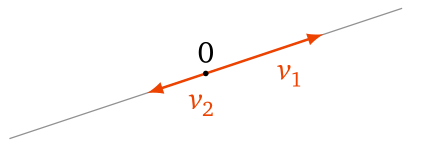
\includegraphics[width=5cm, height=2cm]{./col_r2.png}

     \begin{block}{$\Rr^3$}
       \small
       \small Deux vecteurs dans $\Rr^3$ sont liés (\textbf{linéairement dépendents}) s'ils
       sont \textbf{\alert{colplanaires}} 
     \end{block}
    \centering
    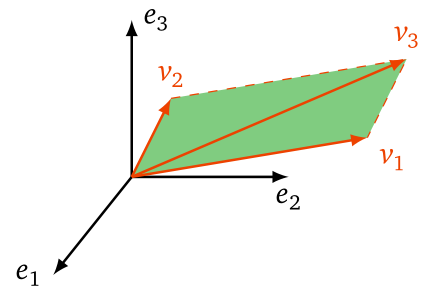
\includegraphics[width=5cm, height=2cm]{./col_r3.png}
\end{frame}
% }}} Interprétation géométrique %
% Mini Exercice {{{ %
\begin{frame}[t]
  \frametitle{Mini Exercice}
  
  \begin{block}{Mini Exercice}
    \begin{itemize}
      \scriptsize
      \item On considère la famille
        \begin{equation}
          \big\{(-1,t)\;,\; (t^2,-t)\big\}
        \end{equation}
        Pour quels valeurs de $t$ cette famille est libre?\\[6pt]
        \scriptsize
      \item Montrer que toute famille \textbf{contenant} une famille liée est
        liée.\\[6pt]
      \item Montrer que toute famille \textbf{contenue} dans une famille libre
        est libre.\\[6pt]
      \item Soit $f: E\longrightarrow F$ une application linéaire
        \textbf{injective}. Montrer alors que si
        $\left\{v_1,v_2,\ldots,v_p\right\}$ est une famille libre de $E$, alors
        $\left\{f(v_1),f(v_2),\ldots, f(v_p)\right\}$ est une famille libre de $F$.
    \end{itemize}
  \end{block}
\end{frame}
% }}} Mini Exercice %
% }}} Famille libre %
% Famille génératrice {{{ %
\subsection{Famille génératrice}

% Définition {{{ %
\begin{frame}[t]
  \frametitle{Famille génératrice}
  \begin{block}{Définition}
    \small
    Soient $v_1,\ldots, v_p$ des vecteurs de $E$. La famille
    $\left\{v_1,\ldots,v_p\right\}$   est une \textbf{\alert{famille
    génératrice}} de l'espace vectoriel $E$ si:

    \begin{equation}
      \forall u\in E\quad u = \lambda_1 v_1 + \lambda_2 v_2 +\ldots + \lambda_p
      v_p
    \end{equation}
  \end{block}
  
  \begin{itemize}
    \small
    \item On dit que la famille $\left\{v_1, \ldots, v_p\right\}$
      \textbf{\alert{engendre}} l'espace vectoriel $E$.\\[4pt]
    \item $E = \text{Vect}(v_1,\ldots, v_p)$
  \end{itemize}

  \begin{block}{Exemple}
    \scriptsize
    Soit $v_1= (1,0,0)$, $v_2=(0,1,0)$ et $v_3=(0,0,1)$.\\[4pt]
    La famille $F=\left\{v_1, v_2, v_3\right\}$ est une famille génératrice de
    $\Rr^3$.\\[4pt]

    \begin{equation*}
      \forall u=(x,y,z)\in \Rr^3\quad  u = x v_1 + y v_2 + z v_3
    \end{equation*}
\end{block}
\end{frame}
% }}} Définition %
% Contre Exemple {{{ %
\begin{frame}[t]
  \frametitle{Exemple 2}
  \begin{block}{Exemple 2}
    \small
    Si on considère  $v_1 = \begin{pmatrix}
     1 \\ 1 \\ 1 
    \end{pmatrix}$ et $v_2 = \begin{pmatrix}
     1 \\ 2 \\ 3 
    \end{pmatrix}$ de $E=\Rr^3$.
   
    Ces deux vecteurs ne forment pas une famille génératice car le vecteur
    $(0,1,0)\notin \left\{v_1, v_2\right\}$  Car 
    \begin{equation}
      \lambda_1 (1,1,1) + \lambda_2 (1, 2, 3) = (0, 1, 0)
    \end{equation}
    
    implique que

    \begin{equation*}
      \left\{
        \begin{array}{lll}
          \lambda_1 + \lambda_2 & =& 0\\[4pt]
          \lambda_1 + 2\lambda_2 & = & 1\\[4pt]
          \lambda_1 + 3\lambda_2 & = & 0
      \end{array}\right.
    \end{equation*}
    Ce système n'admet pas de solution!
  \end{block}
  
\end{frame}
% }}} Contre Exemple %
% Lien enre famille {{{ %
\begin{frame}[t]
  \frametitle{Lien entre famille}
  
  \begin{block}{Proposition }
    \small
    Si $\mathcal{F}=\left\{v_1,v_2,\ldots, v_p\right\}$ est une famille
    \textbf{génératrice} de $E$. alors $\mathcal{F}^{'}=\left\{v_1^{'},
    v_2^{'},\ldots, v_p^{'}\right\}$ est aussi une famille génératrice si et
    seulement si tout élément de $\mathcal{F}$ est une combinaison linéaire de
    $\mathcal{F^{'}}$.
  \end{block}

  \begin{itemize}
    \small
    \item Cette propriété ne change pas le cardinal des familles génératrice. 
    \item Nous cherchons à avoir un nombre minimal de \textbf{générateurs} 
  \end{itemize}
  \pause
  \begin{block}{Réduction}
    \scriptsize
    Si la famille $\left\{v_1,\ldots, v_p\right\}$ engendre $E$. Et si l'un des
    vecteur (par exemple) $v_p$  est une \textbf{cominaison linéaire}  des
    autre alors:

    \begin{equation}
      \left\{v_1,v_2,\ldots, v_{p-1}\right\}
    \end{equation}
    est une famille \textbf{\alert{génératrice}}.
  \end{block}
\end{frame}

% }}} Lien enre famille %
% Mini Exercice {{{ %
\begin{frame}[t]
  \frametitle{Mini Exercice}
 \begin{block}{Mini Exercice}
\scriptsize
   \begin{itemize}
     \item A quelle condition sur $t\in \Rr$, la famille $\left\{ (0,t-1), (t,
       -t), (t^2-t, t-1)\right\}$ est une famille génératrice de $\Rr^2$.\\[4pt]
      \item Même question avec la famille

        \begin{equation*}
          \big\{ (1,0,t), (1,t,t^2), (1,t^2,1)\big\}
        \end{equation*}
 \item Montrer que si $f:E\longrightarrow F$ est une application linéaire
   \textbf{surjective} et que $v_1,\ldots, v_p$ est une famille génératrice de
   $E$.\\

   Alors  $\left\{f(v_1), \ldots, f(v_p)\right\}$ est aussi une famille
   génératrice de $F$.
   \end{itemize}
 \end{block} 
\end{frame}
% }}} Mini Exercice %
% }}} Famille génératrice %
% Base {{{ %
\subsection{Base}
% Définition {{{ %
\begin{frame}[t]
  \frametitle{Introduction}
 \begin{block}{Introduction}
   \begin{itemize}
     \scriptsize
   \item La notion de \textbf{\alert{base}} généralise la notion de
     \textbf{repère}.\\[4pt]
   \item Dans $\Rr^2$, un repère est donné par deux vecteurs non
     \textbf{colinéaires}.\\[4pt]
   \item Dans $\Rr^3$, un repère doit être construit par
     \textbf{trois} vecteurs non colplanaires.
   \end{itemize}
 \end{block} 
 \begin{figure}[htpb]
   \centering
   \begin{tikzpicture}[scale=0.6,>=latex]
     \path[gray,draw,opacity=0.5](0,0)--(6,3);
     \path[gray, draw, opacity=0.5](0,0)--(3,6);
     \path[sexyRed,->,draw] (0,0)--(3,1.5)node[label=below:$v_1$]{};
     \path[sexyRed,->,draw, lightBlue]
       (3,1.5)--(4,2)node[label=below:$\small \lambda v_1$]{};
     \path[sexyRed,->,draw] (0,0)--(1.5,3)node[label=left:$v_2$]{};
     \path[sexyRed,->,draw, lightBlue] (1.5,3)--(2,4)node[label=left:$\small
       \lambda v_2$]{};
   \end{tikzpicture}
   \caption{Illustration Repère $\Rr^2$}%
 \end{figure}
\end{frame}

\begin{frame}{Base}
 \begin{block}{Définition}
   \scriptsize
   Soit $E$ un $\Kk$-espace vectoriel. Une famille $\mathcal{B}=(v_1, v_2,
   \ldots, v_n)$ de vecteurs de $E$ est une \textbf{alert{base}} de $E$ si:
   \begin{itemize}
     \item $\mathcal{B}$ est \structure{\textbf{génératrice}}.\\[2pt]
   \item $\mathcal{B}$ est \alert{\textbf{libre}}.
   \end{itemize}
 \end{block}
 \pause
 \newcommand{\base}{\mathcal{B}}
 \begin{block}{Théorème}
   \scriptsize
   Si $\base = (v_1, v_2,\ldots, v_n)$ une base de l'espace vectoriel $E$.
   Alors tout vecteur de $u \in E$ s'exprime de façon
   \textbf{\alert{unique}} comme combinaison linéaire des éléments de
   $\base$.

   \begin{equation}
     \label{eq:base}
      u = \sum_{i=1}^n \lambda_i v_i
   \end{equation}
 \end{block}
 \scriptsize

 \begin{enumerate}
   \item $(\lambda_1, \ldots,\lambda_n)$ s'appellent des
     \textbf{\alert{coordonées}}  du vecteur $u$ dans la base
     $\base$.\\[4pt]
    \item L'application 
      \begin{equation*}
        \begin{array}{lll}
          \phi : \Kk^n & \longrightarrow & E\\
          (\lambda_1,\ldots,\lambda_n) &\longrightarrow & \sum_{i=1}^n
          \lambda_i v_i
        \end{array}
      \end{equation*}
      est un \textbf{isomorphisme}  entre $\Kk^n$ et $E$.
 \end{enumerate}

\end{frame}
% }}} Définition %
% Exemples {{{ %
\begin{frame}[t]
  \frametitle{Exemples (1)}
 \begin{block}{Base Canonique}
   \scriptsize
   Dans $\Rr^2$, on note $e_1 = (1, 0)$ et $e_2 = (0,1)$ la
   \textbf{\alert{base canonique}}.
 \end{block} 
 \pause
 \begin{block}{Autre base de $\Rr^2$}
  \scriptsize
  On peut générer aussi une base de $\Rr^2$, en considéreant deux vecteurs
  \textbf{non colinéaires}. Par exemple soient $v_1=(3,1)$ et $v_2=(1,2)$.
  Alors $(v_1,v_2)$ forme un base de $\Rr^2$.
 \end{block}
 \begin{figure}[htpb]
   \centering
   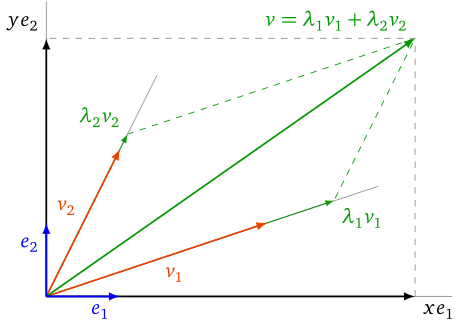
\includegraphics[width=4cm, height=1.6cm]{./simple_base_r2.png}
   \caption{Illustration base $\Rr^2$}%
 \end{figure}
 \begin{block}{Base canonique $\Rr^3$}
   \scriptsize
   On peut aussi donner la base cannonique dans $\Rr^3$ par $v_1=(1,0,0)$,
   $v_2 = (0,1,0)$ et $v_3 = (0,0,1)$.
   
 \end{block}
\end{frame}


\begin{frame}[t]
  \frametitle{Exemple (2)}
  
  \begin{block}{Base non coplanaires}
    \scriptsize
    Soit $v_1 = (1,2,1)$, $v_2 = (2,9,0)$ et $v_3 = (3,3,4)$. Montrer que la
    famille $\mathcal{B} = (v_1, v_2, v_3)$ est une base de $\Rr^3$.
  \end{block}
  \begin{itemize}
    \scriptsize
  \item \textbf{\alert{Génératrice}}: Soit $u=(x,y,z)\in \Rr^3$
    cherchons $\lambda_1,\lambda_2,\lambda_3$ tel que
    \begin{equation*}
      u = \lambda_1 v_1 + \lambda_2 v_2 +\lambda_3 v_3
    \end{equation*}
    \begin{equation*}
      \left\{
        \begin{array}{lll}
          \lambda_1  + 2\lambda_2 + 3\lambda_3 & = & x\\ 
          2\lambda_1  + 9\lambda_2 + 3\lambda_3 & = & y\\ 
          \lambda_1  +  4\lambda_3 & = & z\\ 
        \end{array}
      \right.
    \end{equation*}
  \item \textbf{\alert{Libre}} Soient $\lambda_1,\lambda_2,\lambda_3$ tel que 
    \begin{equation*}
      \lambda_1 v_1 + \lambda_2 v_2 + \lambda_3 v_3 = 0
    \end{equation*}
    \begin{equation*}
      \left\{
        \begin{array}{lll}
          \lambda_1  + 2\lambda_2 + 3\lambda_3 & = & 0\\ 
          2\lambda_1  + 9\lambda_2 + 3\lambda_3 & = & 0\\ 
          \lambda_1  +  4\lambda_3 & = & 0\\ 
        \end{array}
      \right.
    \end{equation*}
  \end{itemize}
\end{frame}
\begin{frame}[t]
  \frametitle{Exemples (3)}
  
  \begin{block}{Base canonique $\Rr^n$}
   Les vecteurs de $\Kk^n$:

   \begin{equation*}
     \scriptsize
     e_1 = \begin{pmatrix}
       1\\0\\ \vdots\\ 0
     \end{pmatrix}
     \quad
     e_2 = \begin{pmatrix}
       0\\1\\ \vdots\\ 0
     \end{pmatrix}
     \quad 
     \ldots
     \quad 
     e_n = \begin{pmatrix}
       0\\0\\ \vdots\\ 1
     \end{pmatrix}
   \end{equation*}
   forment la base \textbf{\alert{canonique}} de $\Kk^n$.
  \end{block}
  \pause

  \begin{block}{Base polynômiale}
   Une base des polynomes de degré $n$ est donnée par:

   \begin{equation*}
     \mathcal{B}  = (1, X, X^2, \ldots, X^n)
   \end{equation*}
  \end{block}
\end{frame}
% }}} Exemples %
% Existence ? {{{ %
\begin{frame}[t]
  \frametitle{Base incomplète}
 \begin{block}{Libre à Base}
   \small
  Soit $E$ un $\Kk$-espace vectoriel admettant une famille
  \textbf{génératrice}.\\

    Toute famille \textbf{libre} $\mathcal{L}$ peut être
    \textbf{\alert{étendue}} à un base.\\[4pt]
      i.e trouver une famille
      $\mathcal{F}$ tel que

      \begin{equation*}
        \mathcal{L} \cup \mathcal{F} \text{ est une base}
      \end{equation*}
    \end{block}

    \pause
    \begin{block}{Génératrice à Base}
      \small
    Toute famille \textbf{génératrice} $\mathcal{L}$  peut être
    \textbf{\alert{réduite}} à une base.\\[4pt]


      i.e Trouver $\mathcal{B} \subset \mathcal{L}$ tel que
      $\mathcal{B}$ est une base.
 \end{block} 
\end{frame}
% }}} Existence ? %
% Mini Exercices {{{ %
\begin{frame}[t]
  \frametitle{Mini Exercice}
 \begin{block}{Mini Exercice}
\begin{enumerate}
  \scriptsize
  \item Soient les vecteurs $v_1=(-1,-3)$, $v_2=(3,3)$, $v_3=(0,0)$,
    $v_4=(2,0)$ et $v_5=(2,6)$.\\[8pt]

    \begin{itemize}
      \scriptsize
      \item Démontrer que $G=(v_1, \ldots, v_5)$ est une famille
        génératrice de $\Rr^2$.\\[4pt]
      \item Extraire une base de  $G$.
    \end{itemize}
  \item Déterminer une base du sous espace vectoriel $E_1$ de $\Rr^3$
    d'équation:
    \begin{equation*}
      x + 3y - 2z = 0
    \end{equation*}
    \begin{itemize}
      \scriptsize
      \item Compléter cette base dans $\Rr^3$.
    \end{itemize}
  \item Même question pour $E_2$ vérifiant les équations:
    \begin{eqnarray*}
      x + 3y -2z &=& 0\\
      y          &=& z
    \end{eqnarray*}
\end{enumerate}  
 \end{block}
\end{frame}
% }}} Mini Exercices %
% }}} Base %
% Dimension {{{ %
\subsection{Dimension}
% Définition {{{ %
\begin{frame}[t]
  \frametitle{Dimension finie}
 \begin{block}{Définition}
   \small
   Un espace vectoriel $E$ admettant une base de cardinal fini est dit de
   \textbf{\alert{dimension finie}}.
 \end{block} 
 \pause

 \begin{block}{Théorème}
   \small
   Toutes les  bases d'un espace vectoriel $E$ de \textbf{dimension finie}  ont
   le même \textbf{\alert{cardinal}}.
 \end{block}
 \pause

 \begin{block}{Définition}
   \small
   Ainsi la \alert{\textbf{dimension}}, notée $\text{dim} E$,  d'un espace
   vectoriel est par définition le cardinal de l'une de ces bases.
 \end{block}
\end{frame}

\begin{frame}[t]
  \frametitle{Exemples}
 \begin{block}{Exemples}
   \small
   \begin{enumerate}
     \item Puisque $\{(1,0), (0,1)\}$ est une base de $\Rr^2$. Alors 
       \begin{equation*}
         \text{dim}\Rr^2 = 2
       \end{equation*}
      \item De même 
        \begin{equation*}
          \text{dim}(\Rr^n) = n
        \end{equation*}
      \item La dimension de l'espace des polynomes de degré $n$ est
        \alert{$n+1$}.
        \begin{equation*}
          \mathcal{B} = \left\{ 1, X, X^2, \ldots, X^n\right\}
        \end{equation*}
      \item $\Rr[X]$ \textbf{n'est pas de dimension finie}.\\[4pt]
      \item $\mathcal{F}(\Rr, \Rr)$ \textbf{n'est pas de dimension finie}.\\[4pt]
   \end{enumerate}
 \end{block} 
\end{frame}
% }}} Définition %
% Résultat s de base {{{ %
\begin{frame}[<+->]
  \frametitle{Complément}
  \begin{block}{Lemme 1}
    \scriptsize
   Soit $E$ un espace vectoriel.  Soit $G$ une famille génératrice de $E$ et
   $\mathcal{L}$ une famille libre alors:
   \begin{equation}
     \text{Card} \mathcal{L} \leq \text{Card} G
   \end{equation}
  \end{block}
  
  \pause

  \begin{block}{Proposition}
    \scriptsize
    Soit $E$ un $\Kk$-espace vectoriel de dimension $\mathbf{n}$

    \begin{enumerate}
      \item Toute famille libre de $E$ à \textbf{\alert{au plus}} $n$
        éléments.\pause

      \item  Toute famille  génératrice de $E$ à \textbf{\alert{au
        moins}}  $n$ éléments.
    \end{enumerate}
  \end{block}
  \pause
  \begin{block}{théorème}
    \scriptsize
    Soient $E$ un $\Kk$-espace vectoriel de dimension $n$ et
    $\mathcal{F}=(v_1,\ldots, v_n) $ une famille de $\alert{n}$
    vecteurs. Alors on as l'équivalence 

    \begin{enumerate}
      \item $\mathcal{F}$ est une base.\\[4pt]
      \item $\mathcal{F}$ est une famille libre.\\[4pt]
      \item $\mathcal{F}$ est une famille génératrice.\\[4pt]
    \end{enumerate}
    
  \end{block}
\end{frame}


\begin{frame}[t]
  \frametitle{Exemple}
 \begin{block}{Question}
   \small
   Pour quelle valeur de $t\in \Rr$, les vecteurs $(v_1, v_2, v_3)$ forment
   une base de $\Rr^3$?
   $$
   v_1 = (1,1,4) \quad v_2 = (1,3,t) \quad v_3=(1,1,t)
   $$
 \end{block} 
 \begin{itemize}
   \small
 \item Puisque on est dans $\Rr^3$ de dimension $\mathbf{3}$, il suffit de
   démontrer que cette famille est soit libre soit génératrice.
 \item En pratique, il est simple de montrer qu'elle est libre.

   \begin{equation*}
     \lambda_1 v_1 + \lambda_2 v_2 +\lambda_3 v_3 = 0
   \end{equation*}

   \begin{equation*}
     \left\{
       \begin{array}{lll}
         \lambda_1  + \lambda_2 + \lambda_3 & = & 0\\
         \lambda_1 + 3\lambda_2 + \lambda_3 & = & 0\\
         4\lambda_1 + t\lambda_2 + t \lambda_3 & = & 0
         
       \end{array}
     \right.
   \end{equation*}
   \begin{equation*}
     \left\{
       \begin{array}{lll}
         \lambda_1  +  \lambda_3 & = & 0\\
         \lambda_2  & = & 0\\
         (t-4) \lambda_3 & = & 0
       \end{array}
     \right.
   \end{equation*}
 \end{itemize}
\end{frame}
% }}} % Résultat s de base %
% Dimension sous espace vectoriel {{{ %
\begin{frame}[t]
  \frametitle{Dimension sous espace vectoriel}
  \begin{block}{Théorème}
    \small
    Soit $E$ un $\Kk$-espace vectoriel de dimension finie.

    \begin{enumerate}
      \item  Tout sous espace vectoriel $F$ de $E$ est de dimension
        finie.\\[4pt]
      \item $\text{dim} F \leq \text{dim} E$\\[4pt]
      \item $F=E \iff \text{dim}F = \text{dim} E$
    \end{enumerate}
  \end{block}
  \pause
  \begin{block}{Théorème des quatre dimensions}
    \small
    Soient $E$ un espace vectoriel de dimension finie, $F$ et $G$ deux
    sous espaces vectoriels de $E$. Alors
    \begin{equation}
      \text{dim}(F + G) = \text{dim}F + \text{dim}G -
      \text{dim}(F\cap G)
    \end{equation}
    \begin{block}{Corollaire}
      \begin{equation*}
        \text{dim}(F\oplus G) = \text{dim}F + \text{dim}G
      \end{equation*}
    \end{block}
  \end{block}
\end{frame}
% }}} Dimension sous espace vectoriel %
% Théorème des quatres dimensions {{{ %
% }}} Théorème des quatres dimensions %
% }}} Dimension %
%}}}
% }}} Full document %

\end{document}
